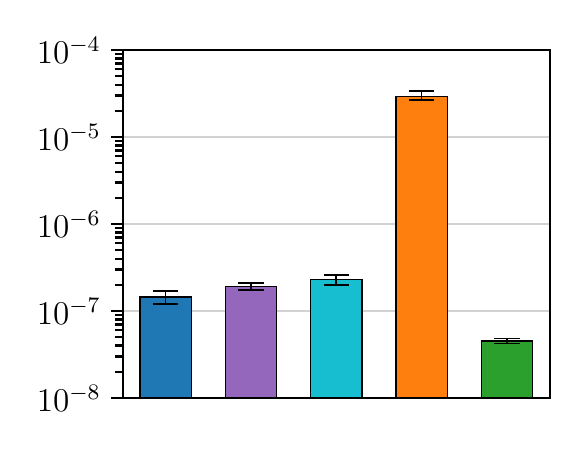
\begin{tikzpicture}
\definecolor{lightgray204}{RGB}{204,204,204}
\definecolor{tabblue}{RGB}{31,119,180}
\definecolor{taborange}{RGB}{255,127,14}
\definecolor{tabpurple}{RGB}{148,103,189}
\definecolor{tabred}{RGB}{214,39,40}
\definecolor{tabcyan}{RGB}{23,190,207}
\definecolor{tabgreen}{RGB}{44,160,44}

\begin{semilogyaxis}[
    line width=0.8pt,
    axis line style={black},
    height=6cm,
    width=7cm,
    xmin=-0.5, xmax=4.5,
    xtick=\empty,
    ymin=1e-8, ymax=1e-4,
    ymajorgrids,
    y grid style={lightgray!70},
    tick align=outside,
    % ylabel={Full Rollout MSE},
    ylabel style={font=\LARGE, color=black},
    tick label style={font=\large, color=black},
    ytick style={color=black, line width=0.8pt},
    ytick={1e-8, 1e-7, 1e-6, 1e-5, 1e-4},
    yticklabels={
        \(10^{-8}\),
        \(10^{-7}\),
        \(10^{-6}\),
        \(10^{-5}\),
        \(10^{-4}\)
    },
    ytick pos=left,
]

% Bars (bottom anchored at ymin=1e-8)
% 0: pointpatch (tab:blue)
\draw[fill=tabblue, draw=black, line width=0.5pt]
    (axis cs:-0.3, 1e-8) rectangle (axis cs:0.3, 1.4541e-7);
% 1: peach_only_ml_and_matprop (tab:purple)
\draw[fill=tabpurple, draw=black, line width=0.5pt]
    (axis cs:0.7, 1e-8) rectangle (axis cs:1.3, 1.9139e-7);
% 2: peach_only_ml_and_sdf (tab:red)
\draw[fill=tabcyan, draw=black, line width=0.5pt]
    (axis cs:1.7, 1e-8) rectangle (axis cs:2.3, 2.2891e-7);
% 3: peach_only_ml (tab:orange)
\draw[fill=taborange, draw=black, line width=0.5pt]
    (axis cs:2.7, 1e-8) rectangle (axis cs:3.3, 2.9077e-5);
% 4: oracle (tab:green)
\draw[fill=tabgreen, draw=black, line width=0.5pt]
    (axis cs:3.7, 1e-8) rectangle (axis cs:4.3, 4.5173e-8);

% Error bars
% 0: pointpatch
\draw[black, semithick] (axis cs:0, 1.2069e-7) -- (axis cs:0, 1.6982e-7);
\draw[black, semithick] (axis cs:-0.15, 1.2069e-7) -- (axis cs:0.15, 1.2069e-7);
\draw[black, semithick] (axis cs:-0.15, 1.6982e-7) -- (axis cs:0.15, 1.6982e-7);
% 1: peach_only_ml_and_matprop
\draw[black, semithick] (axis cs:1, 1.7561e-7) -- (axis cs:1, 2.0982e-7);
\draw[black, semithick] (axis cs:0.85, 1.7561e-7) -- (axis cs:1.15, 1.7561e-7);
\draw[black, semithick] (axis cs:0.85, 2.0982e-7) -- (axis cs:1.15, 2.0982e-7);
% 2: peach_only_ml_and_sdf
\draw[black, semithick] (axis cs:2, 1.9907e-7) -- (axis cs:2, 2.6067e-7);
\draw[black, semithick] (axis cs:1.85, 1.9907e-7) -- (axis cs:2.15, 1.9907e-7);
\draw[black, semithick] (axis cs:1.85, 2.6067e-7) -- (axis cs:2.15, 2.6067e-7);
% 3: peach_only_ml
\draw[black, semithick] (axis cs:3, 2.6516e-5) -- (axis cs:3, 3.3661e-5);
\draw[black, semithick] (axis cs:2.85, 2.6516e-5) -- (axis cs:3.15, 2.6516e-5);
\draw[black, semithick] (axis cs:2.85, 3.3661e-5) -- (axis cs:3.15, 3.3661e-5);
% 4: oracle
\draw[black, semithick] (axis cs:4, 4.2259e-8) -- (axis cs:4, 4.8071e-8);
\draw[black, semithick] (axis cs:3.85, 4.2259e-8) -- (axis cs:4.15, 4.2259e-8);
\draw[black, semithick] (axis cs:3.85, 4.8071e-8) -- (axis cs:4.15, 4.8071e-8);

\end{semilogyaxis}
\end{tikzpicture}